\chapter{Design Pattern}
\section{Design Pattern, cosa sono?}
I \textbf{Design Pattern} sono \textit{soluzioni progettuali generali a problemi ricorrenti}.
Si tratta di una descrizione o modello logico da applicare per risolvere un problema, il quale può presentarsi in diverse situazioni durante le fasi di progettazione e sviluppo del software.

Vanno definiti prima della codifica, questo permette di contenere e ridurre i problemi futuri dello sviluppo di un software.

I design pattern tipicamente mostrano relazioni ed interazioni tra \textit{classi} o \textit{oggetti}, senza specificare le classi applicative finali coinvolte.

\subsection{Come sono costituiti}
Un \textit{design pattern} è costituito da:
\begin{itemize}
	\item \textit{il nome}, costituito da una o più parole che siano rappresentative del pattern stesso;
	\item \textit{il problema}, ovvero la descrizione della situazione alla quale si può applicare il pattern. Può comprendere la descrizione di classi o di problemi di progettazione specifici, come anche una lista di condizioni perché sia necessario l'utilizzo del pattern;
	\item \textit{la soluzione}, che descrive gli elementi che costituiscono il progetto, le relazioni e le relative implicazioni, senza addentrarsi in una specifica implementazione.
	In poche parole bisogna rappresentare un problema astratto e la relativa configurazione di elementi adatta a risolverlo.
	\item \textit{le conseguenze}, risultati e vincoli che derivano dall'applicazione del pattern. 
	Le conseguenze comprendono considerazioni di tempo e di spazio, possono descrivere implicazioni del pattern con alcuni linguaggi di programmazione e l'impatto con il resto del progetto.
	Sono fondamentali in quanto aiutano nella scelta dei pattern.
\end{itemize}
I design pattern possono essere classificati in tre principali categorie\footnote{Le sezioni con \textbf{+} a pedice riguardano design pattern non trattati a lezione}, che risolvono problemi diversi:
\begin{itemize}
	\item Strutturale, delegati alla rappresentazione degli oggetti;
	\item Creazionale, delegati alla gestione della costruzione degli oggetti;
	\item Comportamentale, delegati al comportamento dinamico degli oggetti.
\end{itemize} 
Inoltre esistono pattern architetturali utilizzati più ad alto livello.

\section{Design Pattern Strutturali}
I \textit{design pattern strutturali} sono relativi a come classi ed oggetti sono composti per formare strutture più complesse. 
In generale possiamo distinguere due tipologie di pattern strutturali:
\begin{itemize}
\item basati su \textbf{classi}, i quali utilizzano l'ereditarietà per generare classi che combinano le proprietà di classi base;
\item basati su \textbf{oggetti}, i quali mostrano come comporre gli oggetti al fine di estendere, in fase di esecuzione, le funzionalità di una classe (cosa non possibile nel caso della composizione statica tramite ereditarietà).
\end{itemize}
La maggior parte dei pattern strutturali sono basati sugli oggetti.
Di seguito andremo ad analizzare i principali pattern strutturali conosciuti.

\subsection{Adapter}
Adapter, chiamato anche \textit{wrapper}, è un design pattern strutturale che può essere usato sia su \textit{classi} che su \textit{oggetti}.

Il suo obiettivo è convertire l'interfaccia di una classe in un'altra, in modo da rendere possibile l'interoperabilità tra classi aventi interfacce incompatibili.

Si utilizza quando si vuole usare una classe esistente senza modificarla: questa è la classe da adattare (adaptee). Ci sono due modi per creare la classe \texttt{Adapter}: per ereditarietà o per composizione.

Se si sceglie l'ereditarietà, si utilizza il Class Adapter. Questa variante permette all'\texttt{Adapter} di modificare alcune caratteristiche dell'\texttt{Adaptee}. Tuttavia non funziona se si deve adattare una classe e tutte le sue sottoclassi.

\begin{figure}[H]
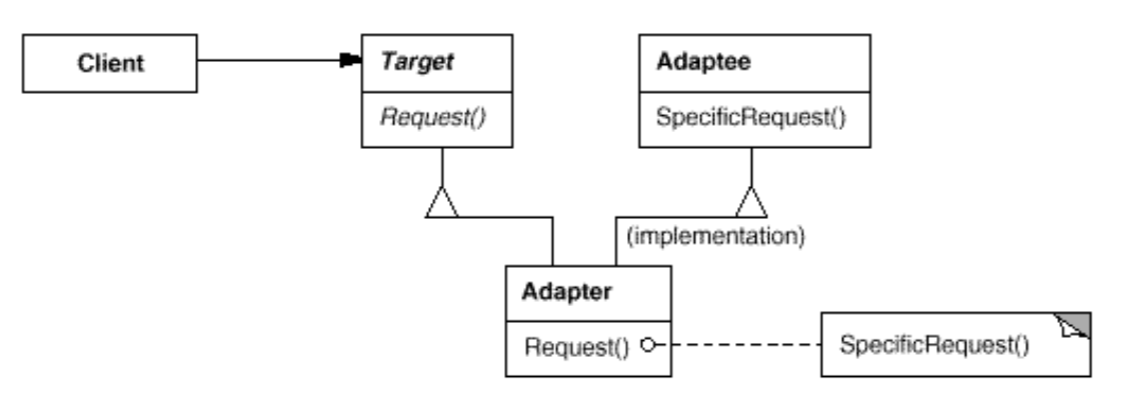
\includegraphics[width=0.8\textwidth]{res/img/DP/classAdapter}
\caption{Class Adapter}
\end{figure}

Se si sceglie la composizione, si utilizza l'Object Adapter. Questa variante invece permette di adattare più tipi (classe e sottoclassi), ma non permette di modificare le caratteristiche dell'\texttt{Adaptee}. Inoltre un oggetto \texttt{adapter} non è sottotipo dell'\texttt{adaptee}.

\begin{figure}[H]
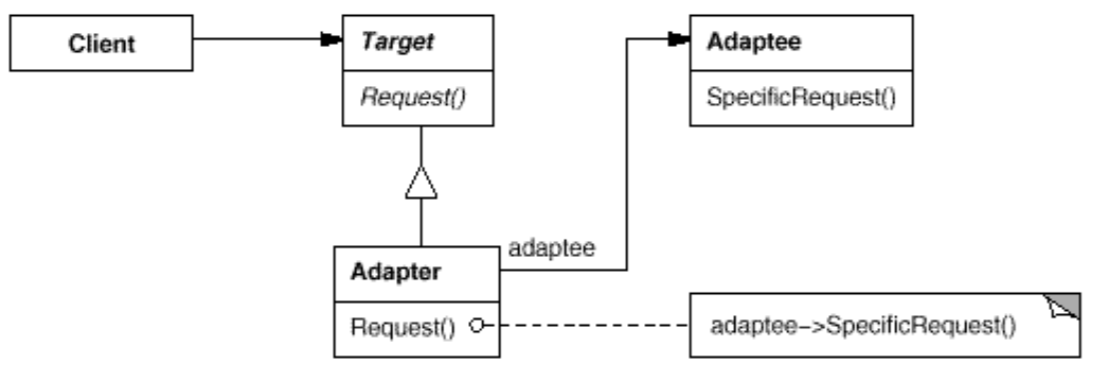
\includegraphics[width=0.8\textwidth]{res/img/DP/objectAdapter}
\caption{Object Adapter}
\end{figure}

L'uso di questo pattern risulta utile quando interfacce di classi differenti devono poter comunicare tra loro, oppure quando si desidera che l'invocazione di un metodo di un oggetto da parte dei client avvenga in maniera "indiretta", ovvero che invece di richiamare il metodo direttamente, si passi attraverso dei metodi "pubblici" che fanno da tramite con l'esterno. 
Questo permette alla classe di subire modifiche future mantenendo la retrocompatibilità.

\subsection{Bridge$_+$}
Il Bridge pattern permette di separare l'interfaccia di una classe (che cosa si può fare con la classe) dalla sua implementazione (come lo fa). 
In tal modo si può usare l'ereditarietà per fare evolvere l'interfaccia o l'implementazione in modo separato.

\subsection{Composite$_+$}
Questo pattern permette di trattare un gruppo di oggetti come se fossero l'istanza di un oggetto singolo. 
Il design pattern Composite organizza gli oggetti in una struttura ad albero, nella quale i nodi sono delle composite e le foglie sono oggetti semplici.\\

È utilizzato per dare la possibilità ai client di manipolare oggetti singoli e composizioni in modo uniforme. \\
Il Composite può essere usato quando i client dovrebbero ignorare la differenza tra oggetti composti e oggetti singoli. 
Se durante lo sviluppo i programmatori scoprono che stanno usando più oggetti nello stesso modo, e spesso il codice per gestirli è molto simile, il Composite rappresenta una buona scelta di rifattorizzazione: in questa situazione, è meno complesso trattare oggetti primitivi e composti in modo omogeneo.

\subsection{Container$_+$}
Il Container pattern permette in certi casi una migliore gestione dell'\textit{incapsulamento}. 
Più che un costrutto, il Container è una buona pratica da seguire per scrivere codice più intelligente e soprattutto sicuro. 

Container consiste nel creare una nuova classe nella quale sarà assegnato un oggetto della nostra classe di partenza come campo della classe, e successivamente la nuova classe creata implementerà un metodo nel quale inseriremo i nuovi passi dell'algoritmo, oltre ad una chiamata all'algoritmo di base tramite l'istanza della classe madre.

\subsection{Decorator}
Il design pattern Decorator consente di aggiungere nuove funzionalità ad oggetti già esistenti. 
Questo viene realizzato costruendo una nuova classe decoratore che "avvolge" l'oggetto originale. 
Al costruttore del decoratore si passa come parametro l'oggetto originale. 
È possibile passarvi un differente decoratore; in questo modo più decoratori possono essere concatenati l'uno all'altro, aggiungendo così in modo incrementale funzionalità alla classe concreta (che è rappresentata dall'ultimo anello della catena).

\begin{figure}[H]
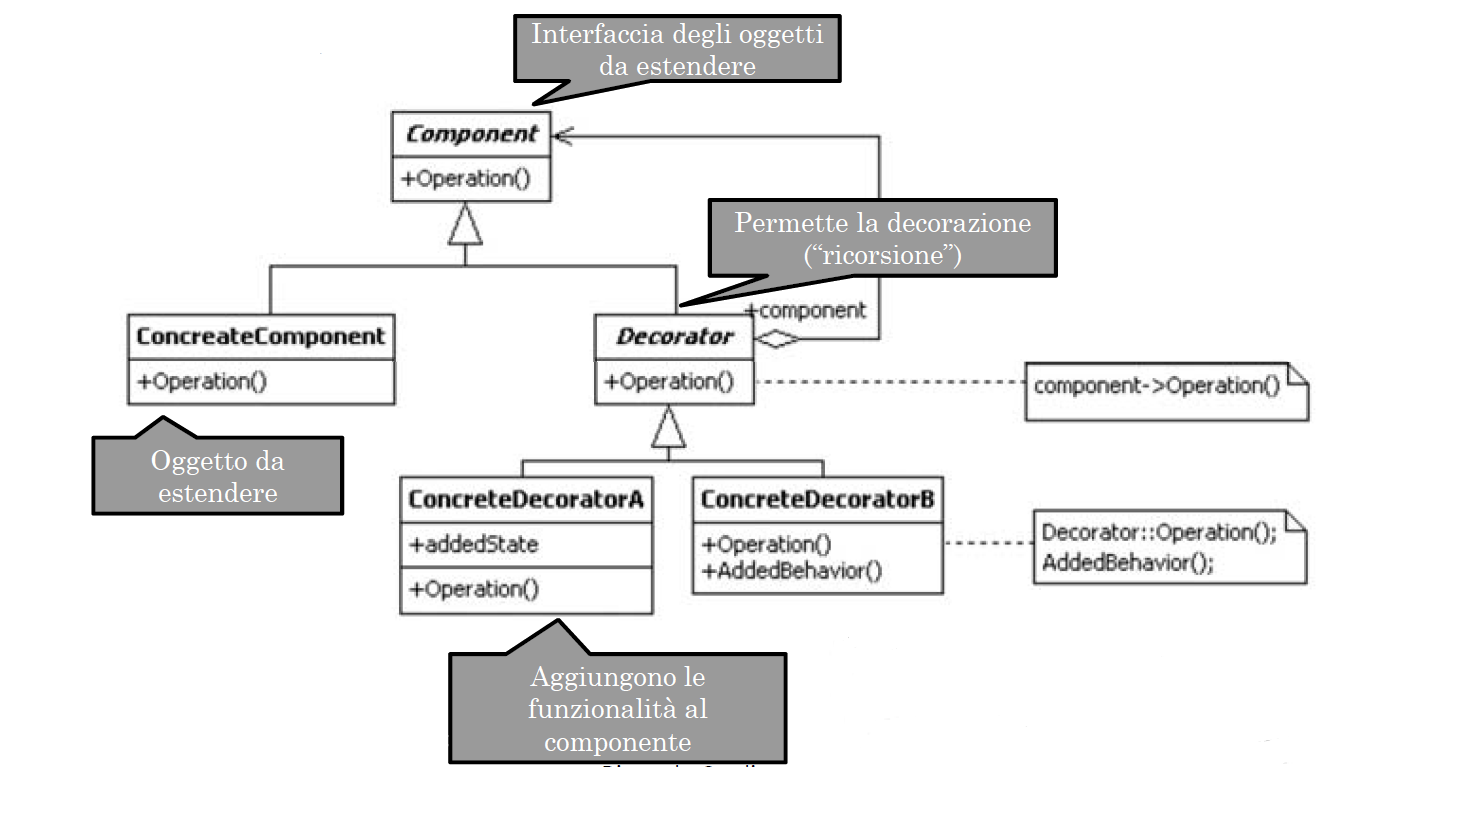
\includegraphics[width=0.8\textwidth]{res/img/DP/decorator}
\caption{Decorator}
\end{figure}

Questo pattern si pone come valida alternativa all'uso dell'ereditarietà singola o multipla. 
Con l'ereditarietà, infatti, l'aggiunta di funzionalità avviene staticamente secondo i legami definiti nella gerarchia di classi e non è possibile ottenere al run-time una combinazione arbitraria delle funzionalità, né la loro aggiunta/rimozione.

Il pattern è ottimo per la sua flessibilità, che permette di aggiungere e rimuovere funzionalità a singoli oggetti a run-time, e per la propensione all'estensibilità del codice, in quanto permette di aggiungere gradualmente le funzionalità senza dover creare classi enormi già in partenza, includendo codice che inizialmente può non essere necessario perché inutilizzato.

\subsection{Façade}
Il design pattern utilizza un oggetto che permette, attraverso un'interfaccia più semplice, l'accesso a sottosistemi che espongono interfacce complesse e molto diverse tra loro, nonché a blocchi di codice complessi.

Il vantaggio è ancora più evidente se questo pattern viene utilizzato in una libreria software, poiché rende indipendente l'implementazione della classe Client dall'implementazione dei vari oggetti Class1, Class2, etc.

\`E un pattern molto utile per la stratificazione di un sistema, se questo utilizza un'architettura a strati.

\begin{figure}[H]
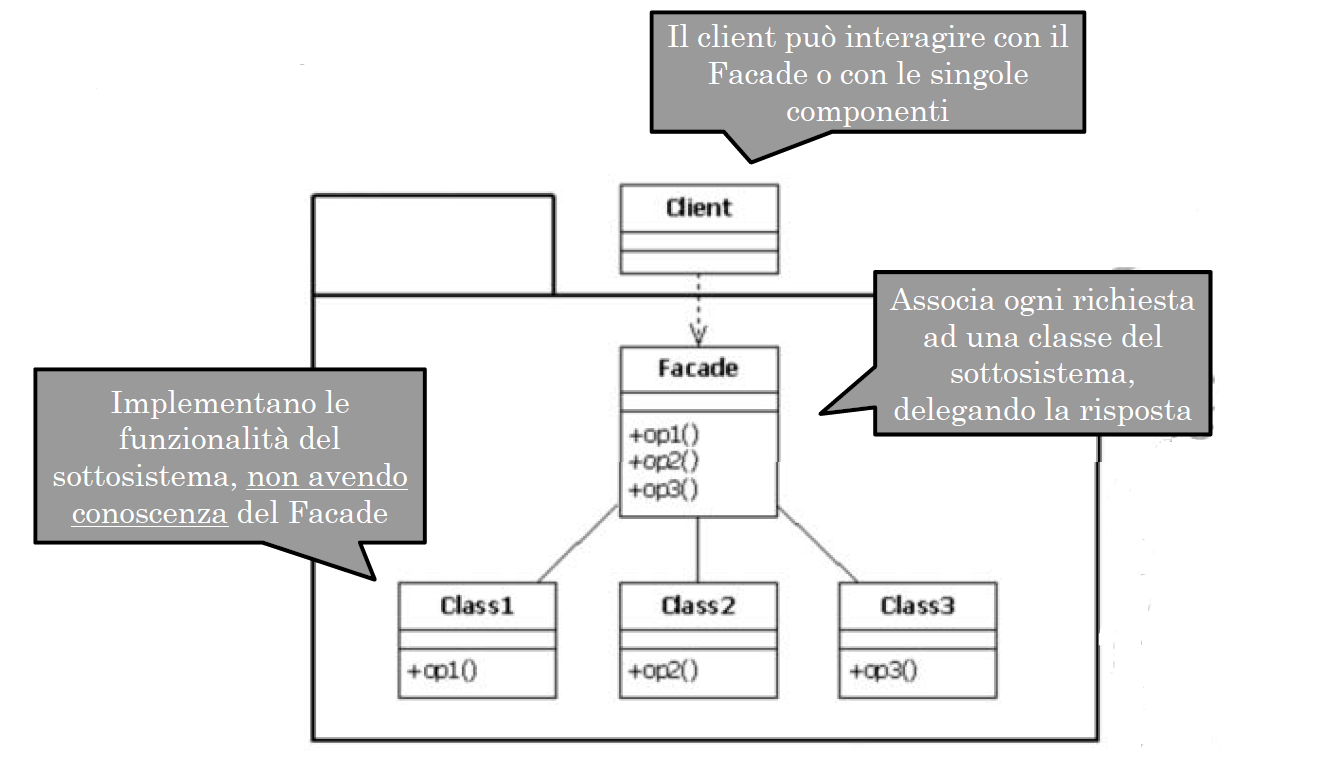
\includegraphics[width=0.8\textwidth]{res/img/DP/facade}
\caption{Façade}
\end{figure}

Nelle librerie standard Java (Java 2 Platform, Standard Edition) questo pattern viene spesso usato; si considerino ad esempio tutte le classi disponibili per fare il rendering del testo o delle forme geometriche, un programmatore può ignorare tutte queste classi e utilizzare unicamente le classi façade (Font e Graphics) che offrono un'interfaccia più semplice e omogenea.

\subsection{Proxy}

Il pattern Proxy crea un surrogato di un oggetto di cui si vuole controllare l'accesso. Un proxy è applicabile nelle seguenti situazioni:
\begin{itemize}
\item Remote proxy: fornisce un rappresentante in locale di un oggetto in un diverso spazio di indirizzamento;
\item Virtual proxy: crea oggetti complessi e pesanti on-demand;
\item Protection proxy: controlla l'accesso all'oggetto originale;
\item Smart reference: rimpiazza il semplice puntatore per svolgere azioni più avanzate, come il reference counting.
\end{itemize}

\begin{figure}[H]
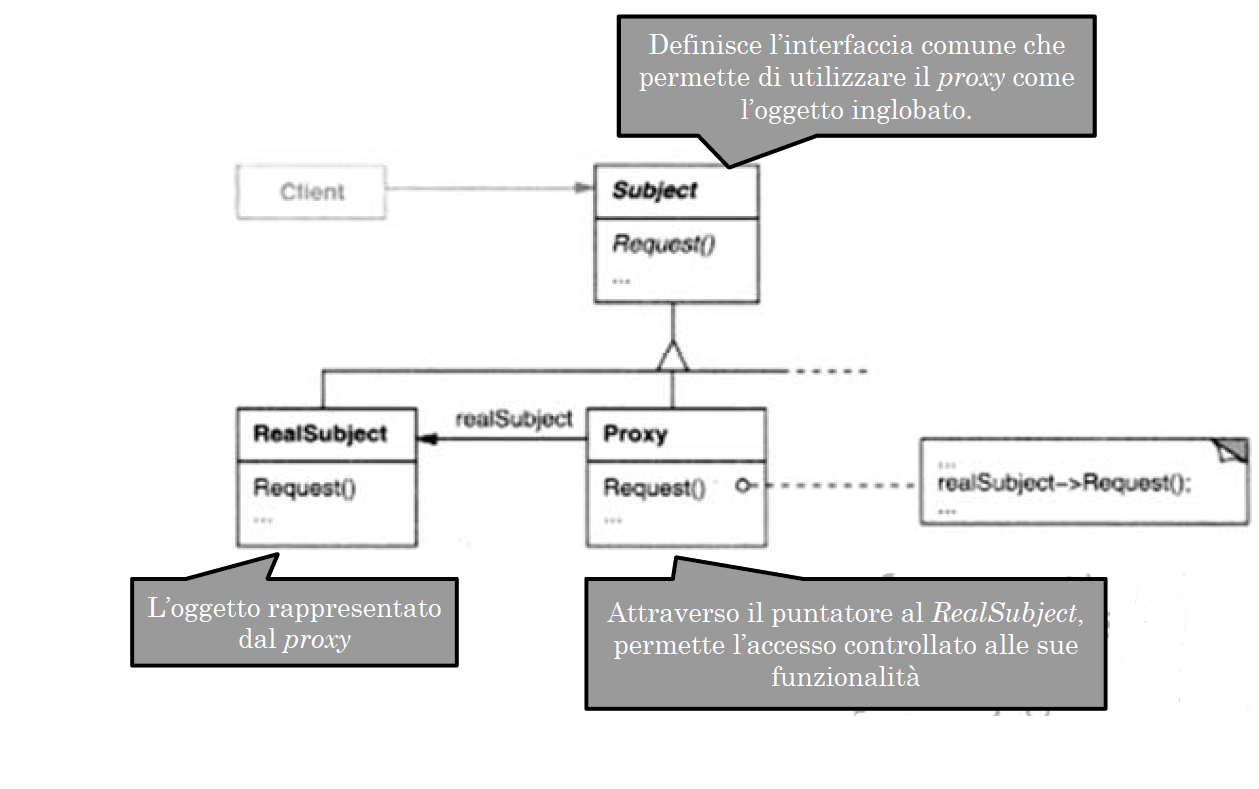
\includegraphics[width=0.8\textwidth]{res/img/DP/proxy}
\caption{Proxy}
\end{figure}

Tipicamente viene creata un'istanza di oggetto complesso, e molteplici oggetti proxy, ognuno dei quali contiene un riferimento al singolo oggetto complesso. 
Ogni operazione svolta sui proxy viene trasmessa all'oggetto originale. 

Una volta che tutte le istanze del proxy sono distrutte, l'oggetto in memoria può essere deallocato.

\subsection{Flyweight$_+$}
Flyweight è un Design pattern che permette di separare la parte variabile di una classe dalla parte che può essere riutilizzata, in modo tale da condividere quest'ultima fra differenti istanze. 
L'oggetto Flyweight deve essere un oggetto immutabile, per permettere la condivisione tra diversi client e thread.

Ad esempio: progettando un word processor si potrebbe creare un oggetto per ogni carattere digitato. 
L'oggetto glifo dovrebbe contenere informazioni come il font, la dimensione e il colore di ogni carattere. 
Il problema è che un testo lungo potrebbe contenere migliaia di caratteri, e oggetti. Il pattern Flyweight risolve il problema creando un nuovo oggetto per memorizzare quelle informazioni che sono condivise da tutti i caratteri con la stessa formattazione. 
Memorizzando le informazioni una volta sola si ha un grosso risparmio di memoria.

\section{Design Pattern Creazionali}
I pattern creazionali forniscono un'astrazione del processo di creazione delle istanze delle classi, favorendo l'indipendenza del sistema dalle modalità di creazione e dai tipi concreti effettivamente generati.

Ci sono due aspetti che caratterizzano i pattern appartenenti a questa categoria:
\begin{itemize}
	\item la capacità di mascherare al client la conoscenza degli oggetti concreti creati, sfruttando tipi astratti per definire le interfacce di riferimento;
	\item la capacità di nascondere le modalità di creazione all'utilizzatore dell'istanza.
\end{itemize}
Queste due caratteristiche conferiscono una notevole flessibilità al processo di creazione, dal momento che ciò che viene creato in generale risulta essere disaccoppiato dal contesto di utilizzo. 
Infatti solo l'oggetto creatore conosce il tipo effettivo dell'istanza e ciò che viene esternamente reso pubblico è unicamente l'interfaccia di riferimento.

\subsection{Abstract factory}

L'Abstract Factory fornisce un'interfaccia per creare famiglie di oggetti connessi o dipendenti tra loro, in modo che non ci sia necessità da parte dei client di specificare i nomi delle classi concrete all'interno del proprio codice.

\begin{figure}[H]
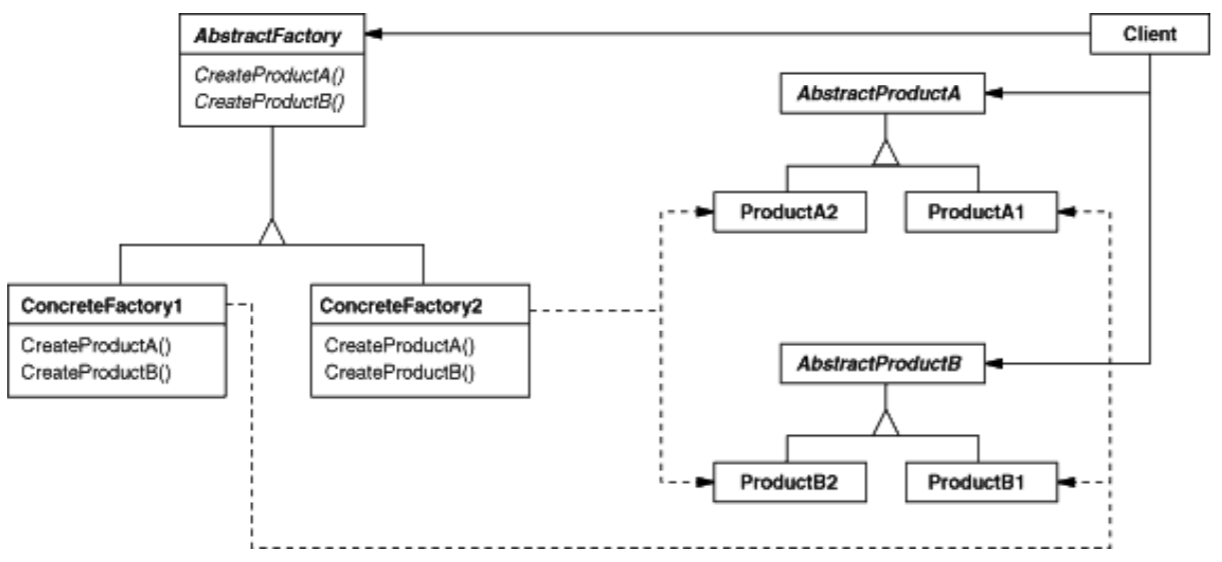
\includegraphics[width=0.9\textwidth]{res/img/DP/abstractFactory}
\caption{Abstract factory}
\end{figure}

In questo modo si permette che un sistema sia indipendente dall'implementazione degli oggetti concreti e che il client, attraverso l'interfaccia, utilizzi diverse famiglie di prodotti.

Questo pattern è utile quando:
\begin{itemize}
	\item si vuole un sistema indipendente da come gli oggetti vengono creati, composti e rappresentati;
	\item si vuole permettere la configurazione del sistema come scelta tra diverse famiglie di prodotti;
	\item si vuole che i prodotti che sono organizzati in famiglie siano vincolati ad essere utilizzati con prodotti della stessa famiglia;
	\item si vuole fornire una libreria di classi mostrando solo le interfacce e nascondendo le implementazioni.
\end{itemize}
\subsection{Builder}

Il design pattern Builder, separa la costruzione di un oggetto complesso dalla sua rappresentazione cosicché il processo di costruzione stesso possa creare diverse rappresentazioni.

\begin{figure}[H]
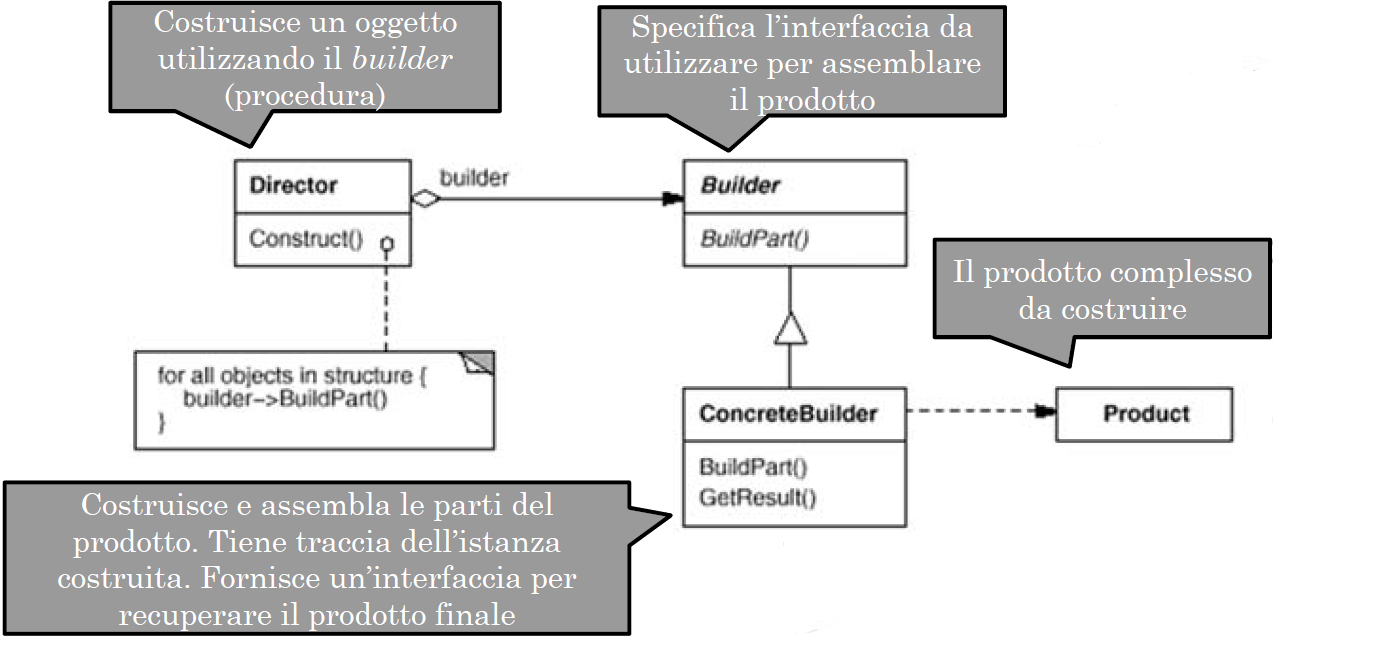
\includegraphics[width=0.9\textwidth]{res/img/DP/builder}
\caption{Builder}
\end{figure}

L'algoritmo per la creazione di un oggetto complesso è indipendente dalle varie parti che costituiscono l'oggetto e da come vengono assemblate.

Ciò ha l'effetto immediato di rendere più semplice la classe, permettendo a una classe \texttt{Builder} separata di focalizzarsi sulla corretta costruzione di un'istanza e lasciando che la classe originale si concentri sul funzionamento degli oggetti. 
Questo è particolarmente utile quando volete assicurarvi che un oggetto sia valido prima di istanziarlo, e non volete che la logica di controllo appaia nei costruttori degli oggetti. 

Un builder permette anche di costruire un oggetto passo-passo, cosa che si può verificare quando si fa il parsing di un testo o si ottengono i parametri da un'interfaccia interattiva.

Spesso il Builder viene utilizzato per la costruzione di un'interfaccia grafica.

\subsection{Factory method$_+$}
il Factory Method indirizza il problema della creazione di oggetti senza specificarne l'esatta classe. Questo pattern raggiunge il suo scopo fornendo un'interfaccia per creare un oggetto, ma lascia che le sottoclassi decidano quale oggetto istanziare.

La creazione di un oggetto può, spesso, richiedere processi complessi la cui collocazione all'interno della classe di composizione potrebbe non essere appropriata. Esso può, inoltre, comportare la duplicazione di codice, richiedere informazioni non accessibili alla classe di composizione, o non provvedere un sufficiente livello di astrazione.
 Il factory method indirizza questi problemi definendo un metodo separato per la creazione degli oggetti; tale metodo può essere ridefinito dalle sottoclassi per definire il tipo derivato di prodotto che verrà effettivamente creato.

Il pattern factory può essere utilizzato quando:
\begin{itemize}
	\item la creazione di un oggetto preclude il suo riuso senza una significativa duplicazione di codice;
	\item la creazione di un oggetto richiede l'accesso ad informazioni o risorse che non dovrebbero essere contenute nella classe di composizione;
	\item la gestione del ciclo di vita degli oggetti gestiti deve essere centralizzata in modo da assicurare un comportamento coerente all'interno dell'applicazione.
\end{itemize}
La gestione del ciclo di vita degli oggetti gestiti deve essere centralizzata in modo da assicurare un comportamento coerente all'interno dell'applicazione.

\subsection{Lazy initialization$_+$}
si dice Lazy initialization (inizializzazione pigra) la tattica di istanziare un oggetto, inizializzare una variabile, effettuare un calcolo od eseguire un processo solo nel momento in cui tale operazione è richiesta.

Tipicamente, questo si ottiene memorizzando in un flag l'avvenimento di un determinato processo. Ogni volta che avviene un certo evento, si esamina il flag. Se questo è abbassato, si continua, altrimenti si inizializza una certa variabile o si istanzia un certo oggetto.

Dal punto di vista dei design pattern, la lazy initialization si usa spesso con un factory method. Questo combina tre idee:
\begin{itemize}
	\item usare un factory method per instanziare una classe;
	\item memorizzare l'istanza di una mappa, in modo tale da poter riprendere la stessa istanza la volta successiva che si richiede la stessa con certi parametri (confronta con un singleton);
	\item usare la lazy initialization per istanziare un oggetto la prima volta che è richiesto.
\end{itemize}

\subsection{Prototype pattern$_+$}
Prototype permette di creare nuovi oggetti clonando un oggetto iniziale, detto appunto prototipo. A differenza di altri pattern come Abstract factory o Factory method permette di specificare nuovi oggetti a tempo d'esecuzione (run-time), utilizzando un gestore di prototipi (prototype manager) per salvare e reperire dinamicamente le istanze degli oggetti desiderati.

Può rivelarsi utile quando:
\begin{itemize}
\item le classi da istanziare sono specificate solamente a tempo d'esecuzione, per cui un codice statico non può occuparsi della creazione dell'oggetto, oppure
\item per evitare di costruire una gerarchia di factory in parallelo a una gerarchia di prodotti, come avviene utilizzando Abstract factory e Factory method, oppure
\item quando le istanze di una classe possono avere soltanto un limitato numero di stati, per cui può essere più conveniente clonare al bisogno il prototipo corrispondente piuttosto che creare l'oggetto e configurarlo ogni volta.
\end{itemize}
\subsection{Singleton}

Singleton ha lo scopo di garantire che di una determinata classe venga creata una e una sola istanza, e di fornire un punto di accesso globale a tale istanza.

\begin{figure}[H]
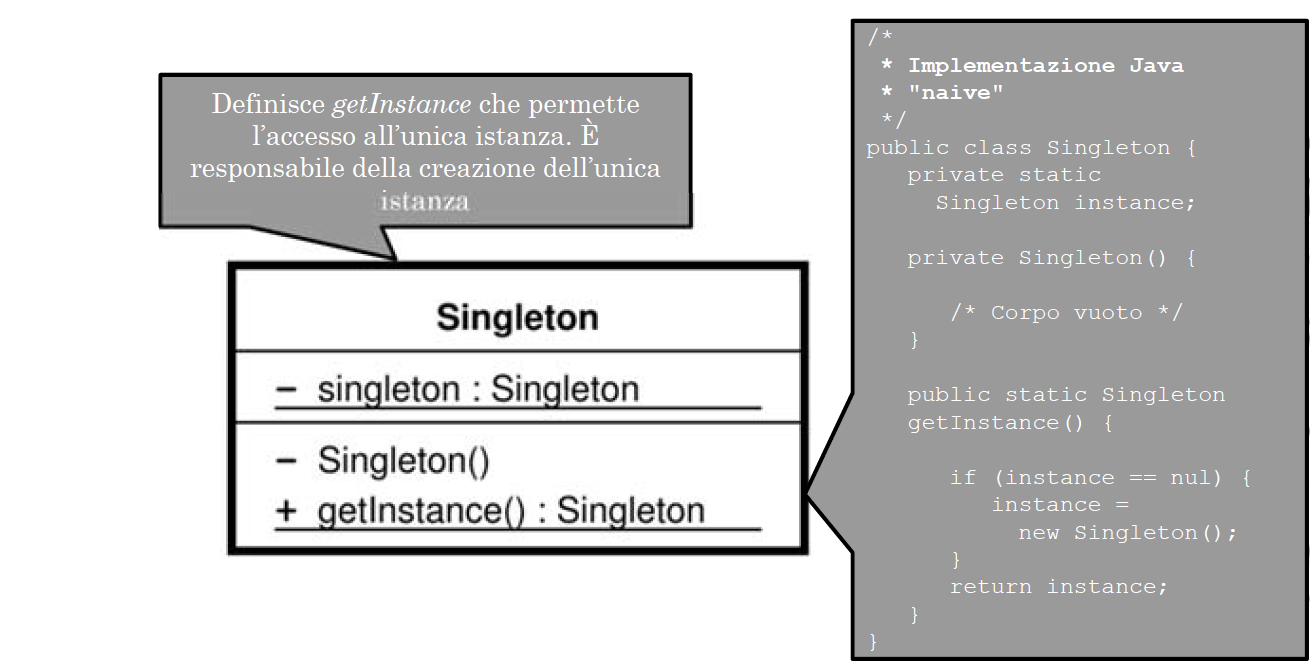
\includegraphics[width=0.9\textwidth]{res/img/DP/singleton}
\caption{Singleton}
\end{figure}

L'implementazione più semplice di questo pattern prevede che la classe singleton abbia un unico costruttore privato, in modo da impedire l'istanziazione diretta della classe. 
La classe fornisce inoltre un metodo "getter" statico che restituisce l'istanza della classe (sempre la stessa), creandola preventivamente o alla prima chiamata del metodo, e memorizzandone il riferimento in un attributo privato anch'esso statico. 

Il secondo approccio si può classificare come basato sul principio della lazy initialization (letteralmente "inizializzazione pigra") in quanto la creazione dell'istanza della classe viene rimandata nel tempo e messa in atto solo quando ciò diventa strettamente necessario (al primo tentativo di uso).

\section{Design Pattern Comportamentali}
I design pattern comportamentali si riferiscono alla distribuzione delle responsabilità tra oggetti tra loro correlati. 
Essi non affrontano unicamente gli aspetti relativi alla struttura degli oggetti e delle classi interagenti, ma si focalizzano soprattutto sulle modalità di comunicazione e collaborazione.

La maggior parte di questi pattern fornisce soluzioni per incapsulare le diverse funzionalità in un oggetto specifico con l'intento di delegare ad esso l'esecuzione del codice vero e proprio. 
Questo approccio permette in generale di eliminare le dipendenze dirette tra i vari oggetti coinvolti, limitando l'accoppiamento e facilitando la possibilità di estendere e modificare il codice senza grossi sforzi.

\subsection{Chain of responsibility$_+$}
Il pattern permette di separare gli oggetti che invocano richieste, dagli oggetti che le gestiscono, dando ad ognuno la possibilità di gestire queste richieste. Viene utilizzato il termine catena perché di fatto la richiesta viene inviata e "segue la catena" di oggetti, passando da uno all'altro, finché non trova quello che la gestisce.

Il pattern è comodo quando non conosciamo a priori quale oggetto è in grado di gestire una determinata richiesta, sia perché effettivamente è sconosciuto staticamente o sia perché l'insieme degli oggetti in grado di gestire richieste cambia dinamicamente a runtime.

\subsection{Command}
Il Command pattern è uno dei design pattern che permette di isolare la porzione di codice che effettua un'azione (eventualmente molto complessa) dal codice che ne richiede l'esecuzione; l'azione è incapsulata nell'oggetto Command.

\begin{figure}[H]
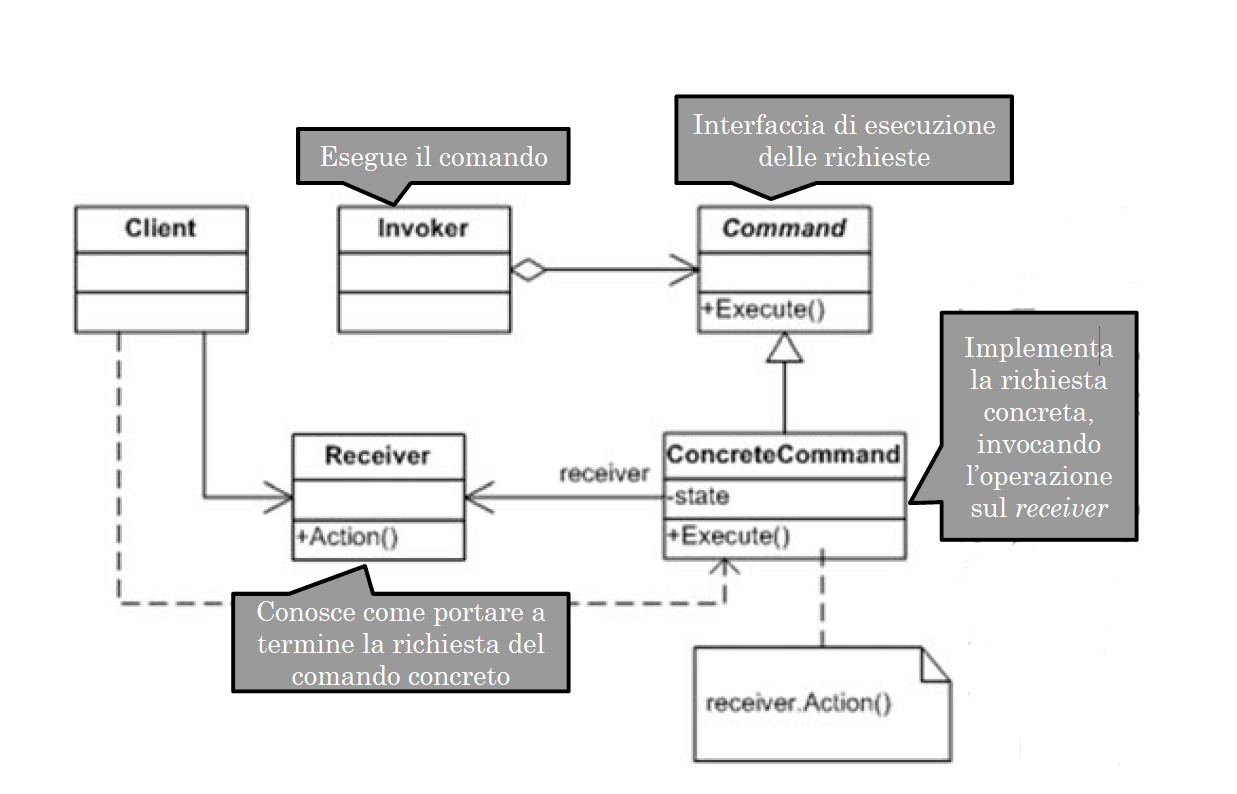
\includegraphics[width=0.9\textwidth]{res/img/DP/command}
\caption{Command}
\end{figure}

L'obiettivo è rendere variabile l'azione del client senza però conoscere i dettagli dell'operazione stessa. 
Altro aspetto importante è che il destinatario della richiesta può non essere deciso staticamente all'atto dell'istanziazione del command ma ricavato a tempo di esecuzione.

\subsection{Interpreter$_+$}
Nella programmazione, l'interpreter viene considerato come un particolare modello di progettazione. 
L'interpreter pattern difatti precisa come valutare le frasi in una determinata lingua o linguaggio. 
L'idea di base è quella di avere una classe per ciascun simbolo (terminale o non terminale) in un linguaggio di programmazione specifico.
L'albero sintattico di una frase nella lingua è quindi un esempio del modello sintattico composito e viene usato per valutare (interpretare) la frase.

\subsection{Iterator}
L'Iterator risolve diversi problemi connessi all'accesso e alla navigazione attraverso gli elementi, in particolare, di una struttura dati contenitrice, senza esporre i dettagli dell'implementazione e della struttura interna del contenitore. 
L'oggetto principale su cui si basa questo design pattern è l'iteratore.

\begin{figure}[H]
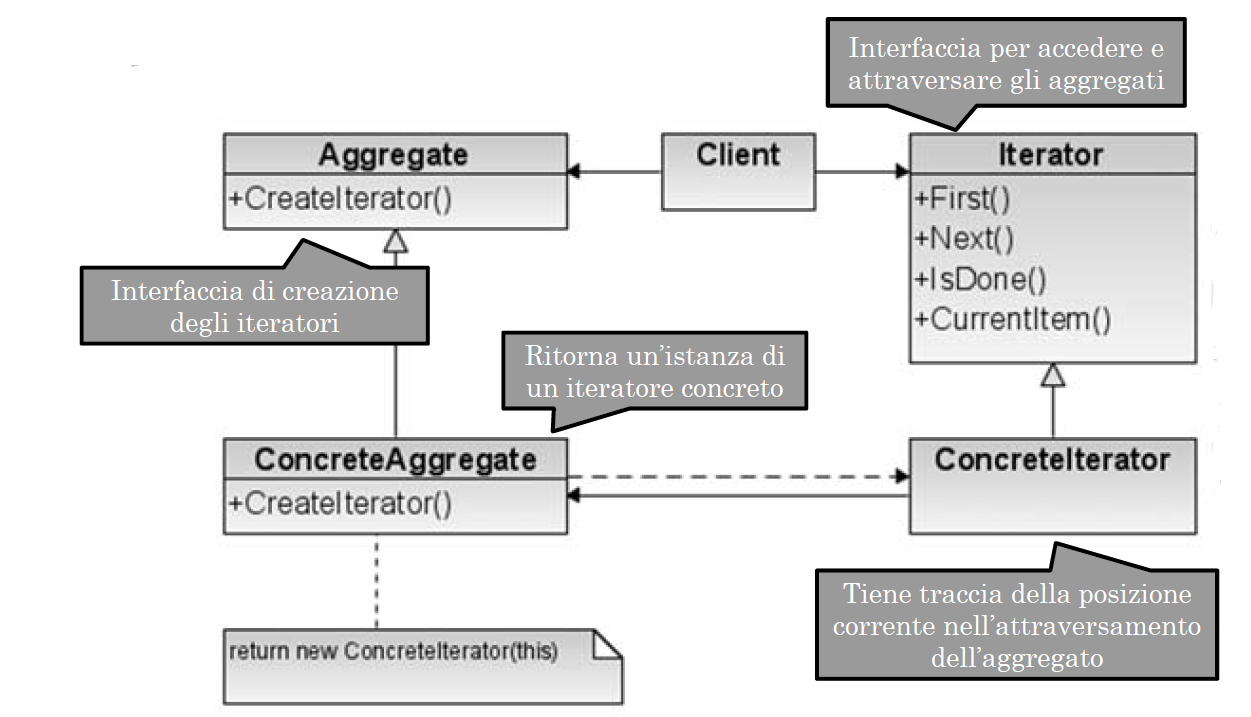
\includegraphics[width=0.9\textwidth]{res/img/DP/iterator}
\caption{Iterator}
\end{figure}

L'idea chiave del pattern Iterator consiste nel trasferire la responsabilità dell'accesso e della navigazione attraverso gli elementi a una classe separata dal contenitore: l'iteratore.

La classe iteratore consente di visitare ad uno ad uno l'insieme degli elementi di un contenitore come se fossero ordinati in una sequenza finita. 
A questo scopo, un oggetto iteratore deve tenere traccia dell'ultimo elemento visitato e deve essere in grado di calcolare qual è l'elemento successivo nella sequenza di attraversamento.

\subsection{Mediator$_+$}
Mediator opera nel contesto delle interazioni tra oggetti, e ha l'intento di disaccoppiare entità del sistema che devono comunicare fra loro. 
Il pattern infatti fa in modo che queste entità non si referenzino reciprocamente, agendo da "mediatore" fra le parti.

Il beneficio principale è il permettere di modificare agilmente le politiche di interazione, poiché le entità coinvolte devono fare riferimento al loro interno solamente al mediatore.

\subsection{Memento$_+$}
Memento (ricorda) l'operazione di estrarre lo stato interno di un oggetto, senza violarne l'incapsulamento, e memorizzarlo, per poterlo poi ripristinare in un momento successivo.

Tipico esempio è l'operazione di Undo, che consente di ripristinare lo stato di uno o più oggetti a come era/erano prima dell'esecuzione di una data operazione.
\subsection{Observer}

Sostanzialmente il pattern si basa su uno o più oggetti, chiamati osservatori o observer, che vengono registrati per gestire un evento che potrebbe essere generato dall'oggetto "osservato", che può essere chiamato soggetto.

\begin{figure}[H]
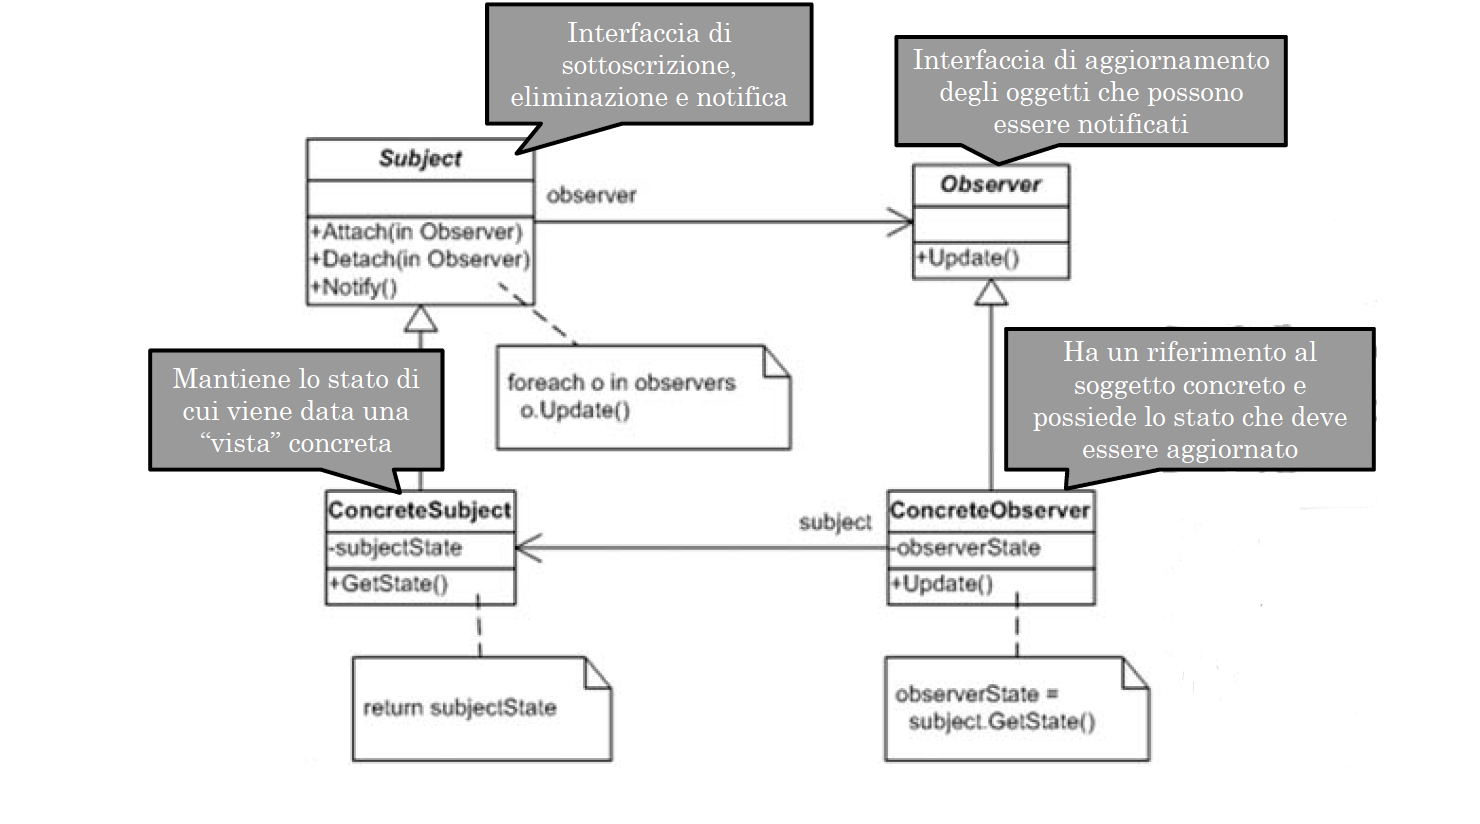
\includegraphics[width=0.9\textwidth]{res/img/DP/observer}
\caption{Observer}
\end{figure}

Uno degli aspetti fondamentali è che tutto il funzionamento dell'observer si basa su meccanismi di callback, implementabili in diversi modi, o tramite funzioni virtuali o tramite puntatori a funzioni passati quali argomenti nel momento della registrazione dell'observer, e spesso a questa funzione vengono passati dei parametri in fase di generazione dell'evento.

\subsection{State$_+$}
Consente ad un oggetto di cambiare il proprio comportamento a run-time in funzione dello stato in cui si trova.

Tra i benefici dell'adozione di questo design pattern vi sono:
\begin{itemize}
	\item Il comportamento associato ad uno stato dipende solo da una classe (ConcreteState);
	\item la logica che implementa il cambiamento di stato viene implementata in una sola classe (Context) piuttosto che con istruzioni condizionali (if o switch) nella classe che implementa il comportamento;
	\item evita stati incoerenti.
\end{itemize}
Tra le conseguenze:
\begin{itemize}
\item Incrementa il numero delle classi.
\end{itemize}

\subsection{Strategy}
L'obiettivo di questa architettura è isolare un algoritmo all'interno di un oggetto, in maniera tale da risultare utile in quelle situazioni dove sia necessario modificare dinamicamente gli algoritmi utilizzati da un'applicazione. 
Si pensi ad esempio alle possibili visite in una struttura ad albero (visita anticipata, simmetrica, posticipata); mediante il pattern strategy è possibile selezionare a tempo di esecuzione una tra le visite ed eseguirla sull'albero per ottenere il risultato voluto.
Anche il design pattern Iterator si basa su questo concetto di isolamento.

\begin{figure}[H]
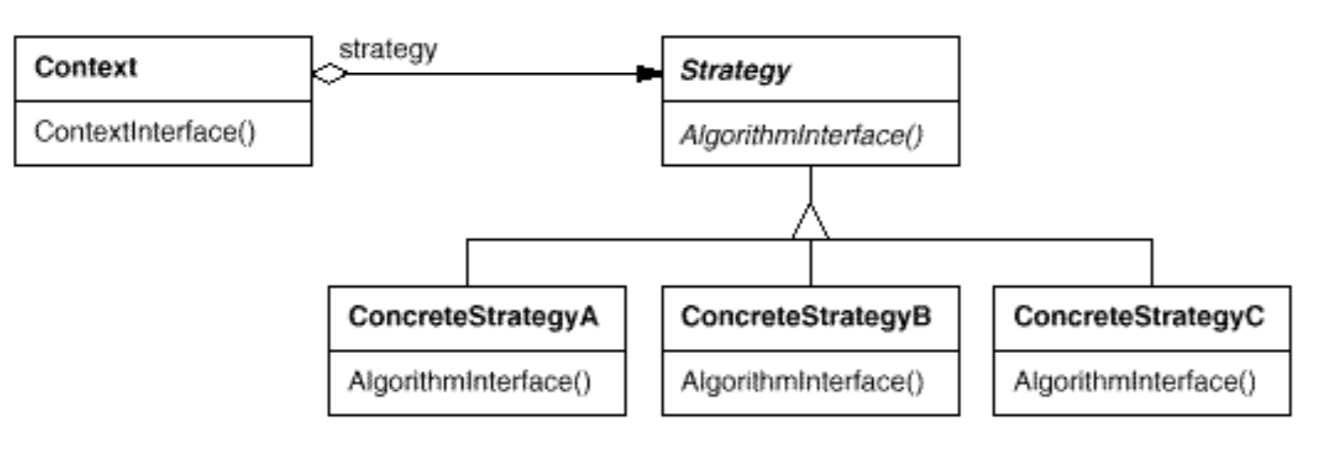
\includegraphics[width=0.9\textwidth]{res/img/DP/strategy}
\caption{Strategy}
\end{figure}

Questo pattern prevede che gli algoritmi siano intercambiabili tra loro, in base ad una specificata condizione, in modalità trasparente al client che ne fa uso. In altre parole, data una famiglia di algoritmi che implementa una certa funzionalità, come può essere ad esempio un algoritmo di visita oppure di ordinamento, essi dovranno esportare sempre la medesima interfaccia, così il client dell'algoritmo non dovrà fare nessuna assunzione su quale sia la strategia istanziata in un particolare istante.

\subsection{Template method}
Questo pattern permette di definire la struttura di un algoritmo lasciando alle sottoclassi il compito di implementarne alcuni passi come preferiscono. In questo modo si può ridefinire e personalizzare parte del comportamento nelle varie sottoclassi senza dover riscrivere più volte il codice in comune.

\begin{figure}[H]
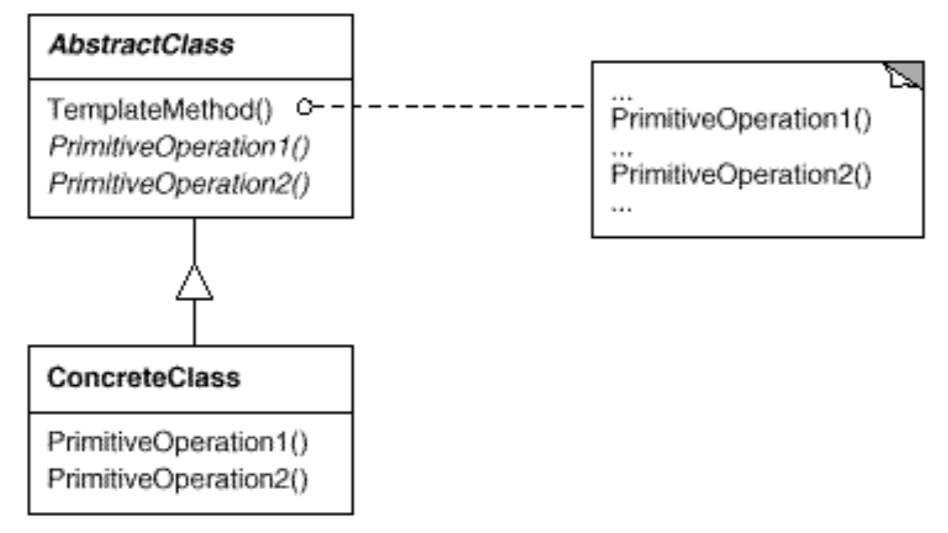
\includegraphics[width=0.9\textwidth]{res/img/DP/template}
\caption{Template method}
\end{figure}

Il pattern è adatto nei seguenti casi:
\begin{itemize}
\item quando si vuole implementare la parte invariante di un algoritmo una volta sola e lasciare che le sottoclassi implementino il comportamento che può variare;
\item quando il comportamento comune di più classi può essere fattorizzato in una classe a parte per evitare di scrivere più volte lo stesso codice;
\item per avere modo di controllare come le sottoclassi ereditano dalla superclasse, facendo in modo che i metodi template chiamino dei metodi "gancio" (hook) e impostarli come unici metodi sovrascrivibili.
\end{itemize}

\subsection{Visitor$_+$}
Permette di separare un algoritmo dalla struttura di oggetti composti a cui è applicato, in modo da poter aggiungere nuove operazioni e comportamenti senza dover modificare la struttura stessa.

Visitor è utile quando:
\begin{itemize}
	\item una struttura di oggetti è costituita da molte classi con interfacce diverse ed è necessario che l'algoritmo esegua su ogni oggetto un'operazione differente a seconda dalla classe concreta dell'oggetto stesso;
	\item è necessario eseguire svariate operazioni indipendenti e non relazionate tra loro sugli oggetti di una struttura composta, ma non si vuole sovraccaricare le interfacce delle loro classi. Riunendo le operazioni correlate in ogni Visitor è possibile inserirle nei programmi solo dove necessario;
	\item le classi che costituiscono la struttura composta sono raramente suscettibili di modifica, ma è necessario aggiungere spesso operazioni sui rispettivi oggetti. Ogni intervento sulle operazioni richiede la modifica o l'estensione di un Visitor, mentre ogni modifica alle classi della struttura vincola alla ridefinizione delle interfacce di tutti i Visitor, compito che può risultare estremamente complesso nei progetti di una certa dimensione.
\end{itemize}

\section{Design Pattern Architetturali}
I pattern architetturali operano ad un livello diverso (e più ampio) rispetto ai design pattern. Descrivono lo schema organizzativo della struttura che caratterizza un sistema software.
In genere questi pattern individuano le parti del sistema a cui sono associate responsabilità omogenee e le relazioni che esistono tra i diversi sottosistemi.
Alcuni esempi di questi pattern sono:

\subsection{Client-server$_+$}
Indica un'architettura di rete nella quale genericamente un computer client o terminale si connette ad un server per la fruizione di un certo servizio, quale ad esempio la condivisione di una certa risorsa hardware/software con altri client, appoggiandosi alla sottostante architettura protocollare.

Più semplicemente, i sistemi client/server sono un'evoluzione dei sistemi basati sulla condivisione semplice delle risorse: la presenza di un server permette ad un certo numero di client di condividerne le risorse, lasciando che sia il server a gestire gli accessi alle risorse per evitare conflitti di utilizzazione tipici dei primi sistemi informatici.

Le reti locali aziendali (LAN), la rete Internet, i sistemi informatici e i sistemi operativi sono organizzati sotto forma di una tipica architettura client-server per la fruizione dei rispettivi servizi.

\subsection{Model-View-Controller MVC}
è un pattern architetturale molto diffuso nello sviluppo di sistemi software, in grado di separare la logica di presentazione dei dati dalla logica di business.

Il componente centrale del MVC, il modello, cattura il comportamento dell'applicazione in termini di dominio del problema, indipendentemente dall'interfaccia utente. Il modello gestisce direttamente i dati, la logica e le regole dell'applicazione.
Una vista può essere una qualsiasi rappresentazione in output di informazioni, come un grafico o un diagramma. Sono possibili viste multiple delle stesse informazioni, come ad esempio un grafico a barre per la gestione e la vista tabellare per l'amministrazione. La terza parte, il controller, accetta l'input e lo converte in comandi per il modello e/o la vista.

l pattern è basato sulla separazione dei compiti fra i componenti software che interpretano tre ruoli principali:
\begin{itemize}
\item il \textbf{model} fornisce i metodi per accedere ai dati utili all'applicazione;
\item il \textbf{view} visualizza i dati contenuti nel model e si occupa dell'interazione con utenti e agenti;
\item il \textbf{controller} riceve i comandi dell'utente (in genere attraverso il view) e li attua modificando lo stato degli altri due componenti.
\end{itemize}
Questo schema, fra l'altro, implica anche la tradizionale separazione fra la logica applicativa (in questo contesto spesso chiamata "logica di business"), a carico del controller e del model, e l'interfaccia utente a carico del view.

I dettagli delle interazioni fra questi tre oggetti software dipendono molto dalle tecnologie usate (linguaggio di programmazione, eventuali librerie, middleware e via dicendo) e dal tipo di applicazione (per esempio se si tratta di un'applicazione web, o di un'applicazione desktop). 
Quasi sempre la relazione fra view e model è descrivibile anche come istanza del pattern Observer. A volte, quando è necessario cambiare il comportamento standard dell'applicazione a seconda delle circostanze, il controller implementa anche il pattern Strategy.

%\subsection{Model-View-Presenter MVP}

\subsection{Model-View-ViewModel}
MVVM è un pattern architetturale e consiste nella separazione degli aspetti della nostra applicazione in tre componenti:
\begin{itemize}
\item Model;
\item View;
\item ViewModel.
\end{itemize}
permettendoci di evitare di mescolare il codice che fornisce la logica a quello che gestisce la UI.
Più precisamente:
\begin{itemize}
	\item Il Model rappresenta il punto di accesso ai dati. Trattasi di una o più classi che leggono dati dal DB, oppure da un servizio Web di qualsivoglia natura;
	\item la View rappresenta la vista dell'applicazione, l'interfaccia grafica che mostrerà i dati;
	\item il ViewModel è il punto di incontro tra la View e il Model: i dati ricevuti da quest'ultimo sono elaborati per essere presentati e passati alla View.
\end{itemize}

Il fulcro del funzionamento di questo pattern è la creazione di un componente, il ViewModel appunto, che rappresenta tutte le informazioni e i comportamenti della corrispondente View. La View si limita infatti, a visualizzare graficamente quanto esposto dal ViewModel, a riflettere in esso i suoi cambi di stato oppure ad attivarne dei comportamenti.

\subsection{Dependency Injection}
Dependency injection è un design pattern il cui scopo è quello di semplificare lo sviluppo e migliorare la testabilità di software di grandi dimensioni.

Per utilizzare tale design pattern è sufficiente dichiarare le dipendenze che un componente necessita (dette anche interface contracts).
Quando il componente verrà istanziato, un iniettore si prenderà carico di risolvere le dipendenze (attuando dunque l'inversione del controllo).
Se è la prima volta che si tenta di risolvere una dipendenza l'injector istanzierà il componente dipendente, lo salverà in un contenitore di istanze e lo ritornerà.
Se non è la prima volta, allora ritornerà la copia salvata nel contenitore.
Una volta risolte tutte le dipendenze, il controllo può tornare al componente applicativo.

Il pattern Dependency Injection coinvolge almeno tre elementi:
\begin{itemize}
\item una componente dipendente;
\item la dichiarazione delle dipendenze del componente, definite come interface contracts;
\item un injector (chiamato anche provider o container) che crea, a richiesta, le istanze delle classi che implementano delle dependency interfaces.
\end{itemize}

% Manca la slide E12 "SOFTWARE ARCHITECTURE PATTERNS"
